\chapter{MEMBANGUN TOPOLOGI (Digitasi On-Screen)}

\begin{enumerate}[\bfseries A.]
  \item \textbf{Digitasi Objek Titik (Point)}
  
  \begin{enumerate}[1.]
    \item Buka file peta dengan memilih File -\textgreater Open, atau membuat layer baru untuk menyimpan titik-titik yang akan dibuat. Biasanya objek titik akan menandakan bidang tertentu tergantung gambar simbol yang dihasilkan.
    
    \item Pilih Map -\textgreater Layer Control atau cukup dengan mengklik ikon 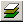
\includegraphics{./resources/052-a-ikon-layer-control} sehingga muncul jendela seperti gambar berikut :
    
    \begin{figure}[H]
      \centering
      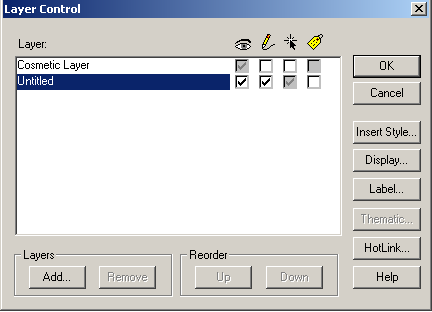
\includegraphics[width=1\textwidth]{./resources/052-jendela-layer-control}
      \caption{Jendela Layer Control}
    \end{figure}
    
    \item Pastikan peta yang akan di digitasi dapat di-edit, perhatikan pada jendela layer control seperti yang ditunjuk tanda panah pada gambar berikut :
    
    \begin{figure}[H]
      \centering
      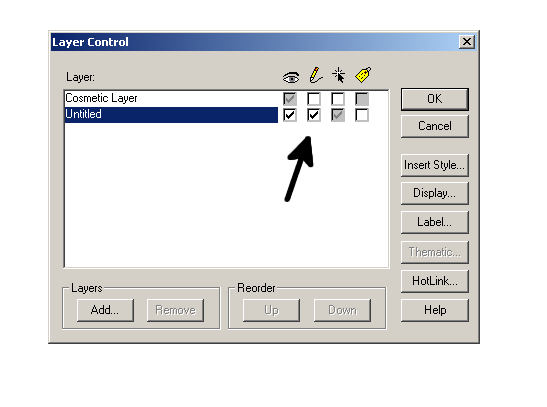
\includegraphics[width=1\textwidth]{./resources/052-b-kondisi-editable}
      \caption{Layer Dapat Diedit}
    \end{figure}
    
    \item Setelah selesai dengan urusan layer, sekarang kita konfigurasi simbolnya, pilih ikon 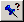
\includegraphics{./resources/054-ikon-setting-simbol} sehingga muncul jendela berikut :
    
    \begin{figure}[H]
      \centering
      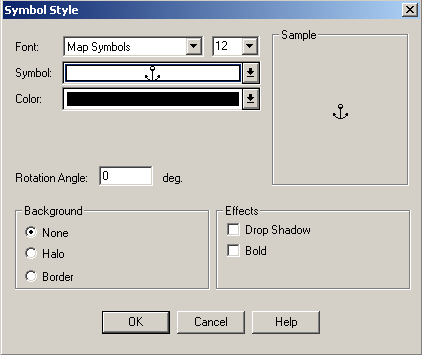
\includegraphics[width=1\textwidth]{./resources/055-jendela-setting-simbol}
      \caption{Jendela Setting Simbol}
    \end{figure}
    
    Kita dapat mengubah jenis huruf dan jenis simbol yang akan digunakan, termasuk disana mengubah ukuran huruf agar dapat ditampilkan lebih jelas.
    
    \item Siap untuk men-digitasi data titik (misal objek Tower BTS atau objek Pelabuhan) dengan menggunakan ikon 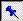
\includegraphics{./resources/053-ikon-simbol} seperti gambar berikut :
    
    \begin{figure}[H]
      \centering
      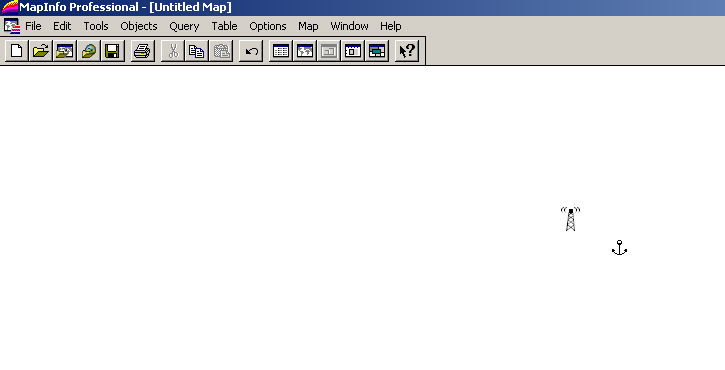
\includegraphics[width=1\textwidth]{./resources/056-contoh-simbol}
      \caption{Contoh Penggambaran Objek Titik}
    \end{figure}
    
    \item Setelah semua data titik selesai di digitasi, simpan data dengan memilih File -\textgreater Save table.
  \end{enumerate}
  
  \item \textbf{Digitasi Objek Garis (Line)}
  
  \begin{enumerate}[1.]
    \item Tambahkan layer bila perlu untuk membuat objek garis (misal objek jalan, atau objek sungai), atau gunakan layer yang sudah ada untuk membuat objek garis.
    
    \item Pilih ikon 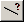
\includegraphics{./resources/057-a-ikon-setting-garis} sehingga muncul jendela untuk dikonfigurasi sesuai kebutuhan, berikut tampilannya :
    
    \begin{figure}[H]
      \centering
      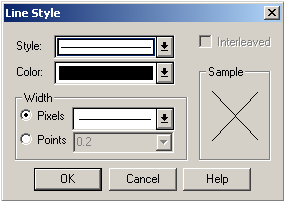
\includegraphics[width=1\textwidth]{./resources/058-jendela-setting-garis}
      \caption{Jendela Konfigurasi Objek Garis}
    \end{figure}
    
    Konfigurasinya meliputi bentuk garis yang akan dibuat, warna yang akan dipilih, serta ukuran ketebalan garis.
    
    \item Siap untuk mendigitasi data garis dengan ikon berikut :
    
    \begin{figure}[H]
      \centering
      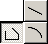
\includegraphics[width=0.5\textwidth]{./resources/059-ikon-garis}
      \caption{Ikon Untuk Menggambar Garis}
    \end{figure}
    
    Untuk menggambar garis sendiri ada 3 (tiga) ikon yang dapat digunakan, yang pertama digunakan untuk menggambar sebuah garis lurus, yang kedua untuk menggambar beberapa garis dalam satu proses (\textit{polyline}), awal pembentukan garis dengan klik kiri, jika ingin mengakhiri pembuatan garisnya, klik ganda tombol kiri \textit{mouse}. Ikon yang ketiga yaitu menggambar garis lengkung.
    
    \item Contoh gambar yang dihasilkan dari ketiga ikon tersebut dapat dilihat pada gambar berikut :
    
    \begin{figure}[H]
      \centering
      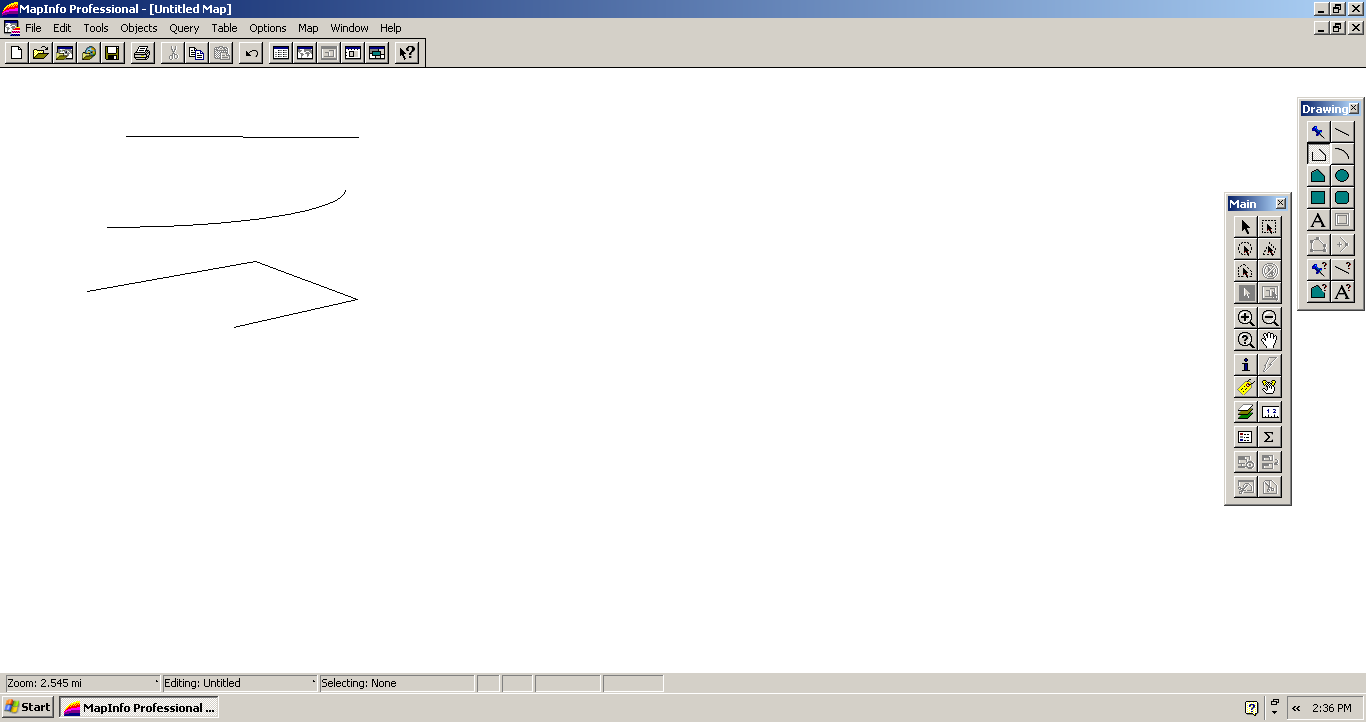
\includegraphics[width=1\textwidth]{./resources/060-contoh-garis}
      \caption{Contoh Hasil Objek Garis}
    \end{figure}
    
    \item Setelah semua data garis selesai digitasi, simpan data dengan memilih \textbf{File} -\textgreater \textbf{Save table}.
  \end{enumerate}
  
  \item \textbf{Digitasi Objek Area (Polygon)}
  
  \begin{enumerate}[1.]
    \item Tambahkan layer bila perlu untuk membuat objek poligon, (misal objek batas Kecamatan, atau objek bidang tanah).
    
    \item Pilih ikon 
\includegraphics{./resources/061-ikon-setting-poligon} sehingga muncul jendela konfigurasi poligon seperti gambar berikut :
    
    \begin{figure}[H]
      \centering
      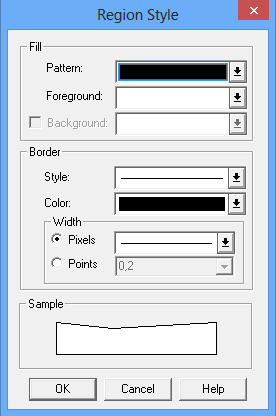
\includegraphics[width=1\textwidth]{./resources/062-jendela-setting-poligon}
      \caption{Jendela Setting Poligon}
    \end{figure}
    
    Kita dapat mengkonfigurasi beberapa hal seperti warna dan jenis isian/arsiran, jenis dan warna garis pinggir, termasuk ketebalan garis pinggir yang akan ditampilkan.
    
    \item Selanjutnya melakukan digitasi data area dengan menggunakan ikon 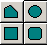
\includegraphics{./resources/063-ikon-poligon}. Cara penggambarannya sama dengan menggambar polyline, klik satu kali di awal titik, dan akhiri dengan klik ganda di titik terakhir.
    
    \item Setelah semua data area sudah selesai digitasi, simpan data dengan memilih Map -\textgreater Save Cosmetic Object. Berikut contoh hasil jadi dari penggambaran objek bidang :
    
    \begin{figure}[H]
      \centering
      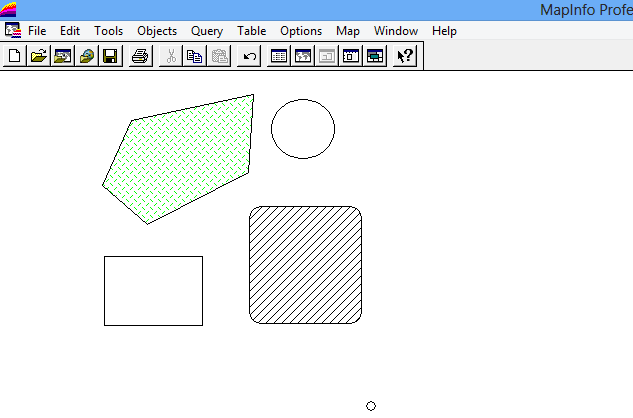
\includegraphics[width=1\textwidth]{./resources/064-hasil-poligon}
      \caption{Contoh Hasil Akhir Penggambaran Objek Area}
    \end{figure}
    
    \item Setelah semua selesai, pilih File -\textgreater Save table.
  \end{enumerate}
  
  \item \textbf{Editing Objek (Feature)}
  
  Untuk meng-edit \textit{feature} setiap objek (biasanya hanya untuk objek garis dan area saja. Objek titik tidak perlu di edit), gunakan prinsip-prinsip dasar pemetaan seperti pada \textbf{BAB 2 PENGENALAN SOFTWARE} sebelumnya. Pastikan \textit{file} yang akan diubah dalam kondisi dapat ter-edit.
\end{enumerate}